\documentclass[12pt]{article} % Định dạng tài liệu kích thước chữ 12pt

\usepackage{polyglossia} % Quản lí ngôn ngữ
\setdefaultlanguage{vietnamese}
\setotherlanguages{english}
\usepackage{fontspec} % Cung cấp khả năng sử dụng ngôn phông chữ OpenType và TrueType
\usepackage{
    amsmath, % Các lệnh toán học
    amsfonts, % Các kí hiệu toán học
    amssymb % Các kí hiệu toán học
}
\usepackage{unicode-math} % Cung cấp hỗ trợ cho các phông chữ toán học Unicode
\setmainfont{STIX Two Text} % Thiết lập phông chữ chính là STIX Two Text
\setmathfont{STIX Two Math} % Thiết lập phông chữ toán học là STIX Two Math

\usepackage[a4paper, left=2cm, right=2cm, top=2cm, bottom=2cm]{geometry} % Định dạng kích thước và lề trang
\usepackage{graphicx} % Hỗ trợ chèn hình ảnh vào tài liệu
\usepackage{xcolor} % Gói màu sắc để tùy chỉnh màu sắc

\usepackage[vietnamese]{hyperref} % Tạo liên kết và tham chiếu trong tài liệu, hỗ trợ tiếng Việt
\hypersetup{
    colorlinks=true, % Kích hoạt màu sắc cho các liên kết
    linkcolor=darkgray,    % Màu của liên kết nội bộ
    citecolor=blue,    % Màu của liên kết tham chiếu
    filecolor=blue,    % Màu của liên kết tập tin
    urlcolor=blue      % Màu của liên kết URL
}
\renewcommand{\sectionautorefname}{Mục} % Đổi tên tự động của các liên kết phần mục từ "Section" thành "Mục"

\usepackage{bookmark} % Tạo mục lục nhanh và chính xác hơn

% Quản lí tài liệu tham khảo với biber 
\usepackage[backend=biber,style=authoryear,sorting=none]{biblatex} 
\addbibresource{references.bib} % Thêm tài liệu tham khảo từ tệp references.bib
\DeclareLanguageMapping{vietnamese}{vietnamese-english} % Định nghĩa ánh xạ ngôn ngữ cho tiếng Việt
\DeclareLanguageMapping{english}{english} % Định nghĩa ánh xạ ngôn ngữ cho tiếng anh

% Định nghĩa môi trường Bài Tập
\newcounter{baitap} % Tạo một bộ đếm mới cho bài tập
\newenvironment{baitap}[1][]{%
    \vspace{10pt} % Khoảng cách từ trên xuống
    \noindent\textsc{Bài tập #1} % Định dạng tiêu đề môi trường bài tập
    \noindent
}{%
    \par
    \vspace{10pt} % Khoảng cách từ dưới lên
}
\newenvironment{baitapcham}[1][]{%
    \vspace{10pt} % Khoảng cách từ trên xuống
    \noindent\textsc{Bài tập. #1} % Định dạng tiêu đề môi trường bài tập
    \noindent
}{%
    \par
    \vspace{10pt} % Khoảng cách từ dưới lên
}
\newenvironment{baitap1}[1][]{%
    \refstepcounter{baitap} % Tăng số đếm của môi trường bài tập 
    \vspace{10pt} % Khoảng cách từ trên xuống
    \noindent\textsc{Bài tập \thebaitap. #1} % Định dạng tiêu đề môi trường bài tập với số đếm
    \noindent
}{%
    \par
    \vspace{10pt} % Khoảng cách từ dưới lên
}


\title{Khai triển \texorpdfstring{\protect\((1+x)^n\)}{(1+x)\textasciicircum n} thành đa thức} % Tiêu đề tài liệu có công thức toán học
% \author{Nguyễn Tấn Nhựt}
\date{}

\allowdisplaybreaks % Cho phép gãy dòng trong các công thức toán học dài

%===============================================

\begin{document}

\maketitle
%\tableofcontents

%%%%%%%%%%

\begin{abstract}
    Bài viết đi sâu vào chi tiết quá trình khai triển biểu thức \((1+x)^n\) thành đa thức. Qui tắc nhân phân phối được áp dụng khéo léo vào các trường hợp đơn giản, kèm theo sơ đồ minh họa phù hợp, làm xuất hiện các hình mẫu cần thiết để diễn giải kết quả cuối cùng của bài toán - định lí nhị thức. Sự xuất hiện tự nhiên của tam giác Pascal, nổi tiếng với khả năng tính các hệ số nhị thức, là minh chứng cho sự khéo léo này. Bài viết không chỉ truyền đạt kiến thức kĩ thuật, mà còn thúc đẩy khả năng tư duy hợp lí và sáng tạo trong nghiên cứu, đồng thời khám phá các bài học sâu sắc từ khi phát hiện đến khi hoàn thiện một vấn đề toán học.
\end{abstract}

%%%%%%%%%%

\section{Dẫn nhập} \label{sec:dan-nhap}

Khai triển biểu thức là biến đổi biểu thức từ dạng này sang dạng khác, thường là từ d
ạng phức tạp sang dạng đơn giản, hoặc từ trừu tượng sang cụ thể. Mục tiêu của việc này là làm cho biểu thức trở nên dễ hiểu hơn và dễ thao tác hơn trong các phép toán. Vấn đề đang xét đến là khai triển biểu thức \((1+x)^n\) thành đa thức. Ví dụ, \((1+x)^2\) được khai triển thành \(1+2x+x^2\). 

Biểu thức \((1+x)^2\) là một trường hợp riêng của biểu thức \((x+y)^2\) với \(y=1\), nhưng khi biết dạng khai triển của biểu thức trước vẫn có thể suy ra dạng khai triển của biểu thức sau. Để nhìn thấy điều này, với \(x\ne 0\), tôi đã quan sát 
    \begin{align*}
        (x+y)^2
            &=x^2\left(1+\frac{y}{x}\right)^2 \\
            &=x^2\left[1+2\left(\frac{y}{x}\right)+\left(\frac{y}{x}\right)^2\right] \\
            &=x^2+2xy+y^2.
    \end{align*}
Tương tự như vậy, tôi cũng có 
\[(x+y)^n=x^n\left(1+\frac{y}{x}\right)^n,\]
do đó, việc nghiên cứu dạng khai triển của \((1+x)^n\) không làm mất tính tổng quát của bài toán.

Để ngắn gọn và đạt hiệu quả truyền đạt cao hơn trong khi lập luận, tôi gọi \(p_n\) là dạng khai triển của \((1+x)^n\). Ví dụ, \(p_2\) là \(1+2x+x^2\). Khi nói đến \(p_2\), tôi liền nghĩ đến \(1+2x+x^2\), tôi không nghĩ đến \((1+x)^2\) hay các dạng trung gian. Để bài toán được hoàn thiện, tôi đã xác định hai trường hợp đặc biệt, \((1+x)^0=1\) theo qui ước và \((1+x)^1=1+x\) là tầm thường. Kể từ đây, \(n\) được hiểu là một số nguyên không âm, \(p_0=1\) và \(p_1=1+x\).

Gọi việc khai triển biểu thức \((1+x)^n\) hay \((x+y)^n\) là \emph{khai triển nhị thức} vì biểu thức \(1+x\) hay \(x+y\) có dạng nhị thức. Mục tiêu là xác định \(p_n\) và kết quả này được gọi là \emph{định lí nhị thức}.

%%%%%%%%%%%

\section{Dáng điệu \texorpdfstring{\protect\(p_n\)}{dạng khai tiển lũy thừa nhị thức}}
Áp dụng luật phân phối của phép nhân đối với phép cộng là cách trực tiếp tìm ra \(p_n\). Tôi bắt đầu với trường hợp đơn giản nhất, tìm \(p_2\),
\begin{align*}
    (1+x)^2
        & = (1+x)(1+x) \\
        & = (1+x)1 + (1+x)x \\
        & = 1 + x + x +x^2 \\
        & = 1 + 2x + x^2.
\end{align*}
Ở đây, nhị thức thứ nhất được nhân phân phối với từng hạng tử của nhị thức thứ hai. Nói một cách hình thức, việc tìm \(p_2\) được thực hiện bằng cách nhân phân phối \(1+x\) với \(p_1\). Quá trình nhân phân phối này được mô tả thông qua sơ đồ trong \autoref{fig:so-do-nhan-phan-phoi-hai-nhi-thuc}.

\begin{figure}[htbp]
    \centering
    \includegraphics*[scale=1]{./tex-images/so-do-nhan-phan-phoi-hai-nhi-thuc/so-do-nhan-phan-phoi-hai-nhi-thuc.pdf}
    \caption{Sơ đồ mô tả nhân phân phối \(1+x\) với \(p_1\) thu được \(p_2\).}
    \label{fig:so-do-nhan-phan-phoi-hai-nhi-thuc}
\end{figure}

Để tìm \(p_3\), thay vì trực tiếp nhân phân phối ba nhị thức, tôi sẽ nhân phân phối \(1+x\) với \(p_2\),
\begin{align*}
    (1+x)^3
        & = (1+x)(1+x)^2 \\
        & = (1+x)(1+2x+x^2) \\
        & = (1+x)1+(1+x)2x+(1+x)x^2\\
        & = 1 + x + 2x + 2x^2 + x^2 +x^3\\
        & = 1 + 3x + 3x^2 + x^3.
\end{align*}
Quá trình nhân phân phối này cũng được mô tả thông qua sơ đồ trong \autoref{fig:phan_phoi_nhi_thuc_voi_tam_thuc}.
\begin{figure}[htbp]
    \centering
    \includegraphics*[scale=1]{./tex-images/so-do-nhan-phan-phoi-nhi-thuc-voi-tam-thuc/so-do-nhan-phan-phoi-nhi-thuc-voi-tam-thuc.pdf}
    \caption{Sơ đồ mô tả nhân phân phối \(1+x\) với \(p_2\) thu được \(p_3\).}
    \label{fig:so-do-nhan-phan-phoi-nhi-thuc-voi-tam-thuc}
\end{figure}

Tổng quát, để tìm \(p_n\), tôi áp dụng qui tắc nhân phân phối cho biểu thức \((1+x)p_{n-1}\). Minh họa chi tiết cho thủ thuật này được thể hiện qua tháp tìm \(p_5\) ở \autoref{fig:thap-nhan-phan-phoi-den-n-bang-5}. Tháp này giúp tôi nhận ra các hình mẫu góp phần vào việc xác định \(p_n\). 

Để chuẩn bị cho việc viết ra các hình mẫu này, tôi cần một số kí hiệu phù hợp. Gọi \(\binom{n}{j}\), với \(0\leq j \leq n\), là hệ số của \(x^j\) trong \(p_n\), và qui ước \(\binom{n}{0}=\binom{n}{n}=1\) với mọi \(n\). Qui ước này hợp lí vì, với mọi \(n\), \(p_n\) có duy nhất hạng tử \(1\) và duy nhất hạng tử \(x^n\), mà \(\binom{n}{0}\) là hệ số của \(x^0\), \(x_0=1\) theo qui ước, còn \(\binom{n}{n}\) là hệ số của \(x^n\). Các hệ số \(\binom{n}{j}\) sẽ được gọi là các \emph{hệ số nhị thức}. Ví dụ, \(p_2\) và \(p_3\) được viết lại bởi các kí hiệu này là \(p_2=\binom{2}{0}+\binom{2}{1}x+\binom{2}{2}x^2\) và \(p_3=\binom{3}{0}+\binom{3}{1}x+\binom{3}{2}x^2+\binom{3}{3}x^3\).

Tháp trong \autoref{fig:thap-nhan-phan-phoi-den-n-bang-5} gợi ý rằng, với mọi số nguyên không âm \(n\), \(p_n\) có thể được viết như sau
\begin{align}
    p_n=\binom{n}{0}+\binom{n}{1}x+\cdots+\binom{n}{n-1}x^{n-1}+\binom{n}{n}x^n \label{eq:dang-khai-trien}
\end{align}
Bên cạnh đó, với \(1\leq j\leq n\), tôi có 
\begin{align}
    \binom{n}{j}=\binom{n-1}{j-1}+\binom{n-1}{j}, \label{eq:tinh-he-so-nhi-thuc-theo-chieu-doc}
\end{align}
và với \(0\leq j\leq n\), tôi có 
\begin{align}
    \binom{n}{j}=\binom{n}{n-j}. \label{eq:tinh-doi-xung}
\end{align}

\begin{figure}[htbp]
    \centering
    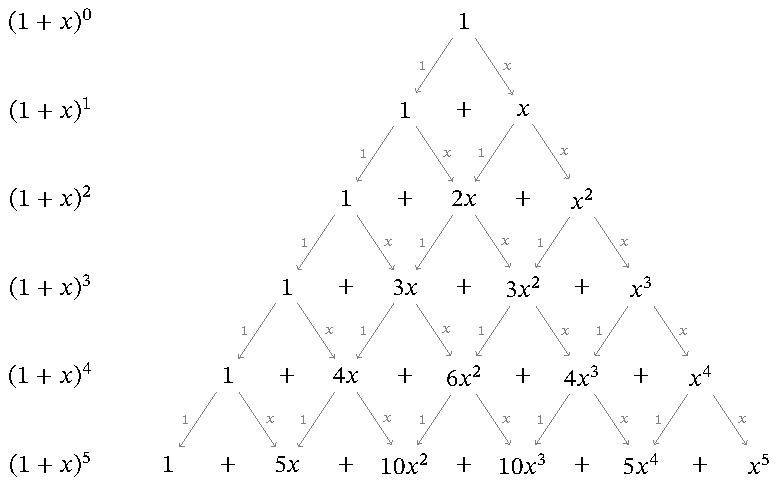
\includegraphics[scale=1]{./tex-images/thap-nhan-phan-phoi-den-n-bang-5/thap-nhan-phan-phoi-den-n-bang-5.pdf}
    \caption{Tháp mô tả quá trình nhân phân phối \(1+x\) với \(p_0\), \(p_1\), \(p_2\), \(p_3\), \(p_4\) thu được \(p_5\).}
    \label{fig:thap-nhan-phan-phoi-den-n-bang-5}
\end{figure} 

Để chứng minh các công thức trên, tôi sử dụng phương pháp qui nạp. Lấy \(p_2=1+2x+x^2\) và \(p_3=1+3x+3x^2+x^3\) làm cơ sở qui nạp, vì dễ dàng kiểm chứng chúng thỏa mãn các công thức \eqref{eq:dang-khai-trien}, \eqref{eq:tinh-he-so-nhi-thuc-theo-chieu-doc} và \eqref{eq:tinh-doi-xung}. Xem \eqref{eq:dang-khai-trien} và \eqref{eq:tinh-he-so-nhi-thuc-theo-chieu-doc} là các giải thiết qui nạp, áp dụng chúng để có
\begin{align*}
    (1+x)p_{n}
        & =  (1+x)\binom{n}{0}+(1+x)\binom{n}{1}x+\cdots+(1+x)\binom{n}{n-1}x^{n-1}+(1+x)\binom{n}{n}x^n\\
        & = \binom{n}{0} + \left[\binom{n}{0}+\binom{n}{1}\right] x + \cdots + \left[\binom{n}{n-1}+\binom{n}{n}\right]x^{n}+\binom{n}{n}x^{n+1} \\
        & = \binom{n+1}{0} + \binom{n+1}{1}x+\cdots+\binom{n+1}{n}x^n+\binom{n+1}{n+1}x^{n+1}.
\end{align*}
Đây chính là kết luận qui nạp cần rút ra cho hai công thức \eqref{eq:dang-khai-trien} và \eqref{eq:tinh-he-so-nhi-thuc-theo-chieu-doc}, với lưu ý \(\binom{n+1}{0}\) được viết thay cho \(\binom{n}{0}\) là vì cả hai đều bằng \(1\) theo qui ước, giải thích tương tự cho trường hợp còn lại. 

Áp dụng công thức \eqref{eq:tinh-he-so-nhi-thuc-theo-chieu-doc}, mà ở trên vừa chứng minh xong, để chỉ ra
\begin{align*}
    \binom{n+1}{j}=\binom{n}{j-1}+\binom{n}{j}
\end{align*}
và
\begin{align*}
    \binom{n+1}{n+1-j}=\binom{n}{n-j}+\binom{n}{n+1-j}.
\end{align*}
Theo giả thiết qui nạp \eqref{eq:tinh-doi-xung}, nếu \(0\leq j\leq n\) thì \(\binom{n}{j}=\binom{n}{n-j}\). Điều này cũng ngụ ý rằng nếu \(0\leq j-1\leq n\) thì \(\binom{n}{j-1}=\binom{n}{n-(j-1)}\). Vậy, suy ra
\begin{align*}
    \binom{n+1}{j}=\binom{n+1}{n+1-j}.
\end{align*}
Đây chính là kết luận qui nạp dành cho công thức \eqref{eq:tinh-doi-xung}. \(\square\)

Kết thúc mục này tại đây, tôi tạm kết luận rằng, khi viết dưới dạng tổng xích-mờ\footnote{sigma}, \(p_n\) có dạng
\[p_n=\sum_{j=0}^n\binom{n}{j}x^j.\] 
Tuy nhiên, bạn nên lưu ý rằng, công thức này vẫn chưa hoàn chỉnh, vì các hệ số nhị thức \(\binom{n}{j}\), ngoài hai tính chất \eqref{eq:tinh-he-so-nhi-thuc-theo-chieu-doc} và \eqref{eq:tinh-doi-xung}, vẫn chưa có một công thức tường minh để tính toán chúng. Cả hai công thức này đều thể hiện tính chất truy hồi hoặc đối xứng của các hệ số nhị thức, nhưng không cung cấp một cách tính trực tiếp và rõ ràng các giá trị của chúng. Trong mục tiếp theo, tôi sẽ cố gắng giải quyết vấn đề này.

%%%%%%%%%%

\section{Dáng điệu \texorpdfstring{\protect\(\binom{n}{j}\)}{hệ số nhị thức}}

Nhờ vào công thức \eqref{eq:tinh-he-so-nhi-thuc-theo-chieu-doc}, tôi có thể tiếp tục mở rộng chân tháp trong \autoref{fig:thap-nhan-phan-phoi-den-n-bang-5}. Ví dụ, tôi có thể lần lượt viết thêm các \(p_6\), \(p_7\), \(p_8\), và \(p_9\). Để đơn giản, lần này tôi chỉ viết các hệ số, kết quả được hiển thị trong \autoref{fig:thap-he-so-nhi-thuc-den-n-bang-9}. Thay thế các con số cụ thể bằng các kí hiệu, tôi có được \autoref{fig:thap-he-so-nhi-thuc-dang-ki-hieu-den-n-bang-9}, trong đó các kí hiệu giúp dễ dàng theo dõi các qui luật hình thành tháp mà đôi khi các con số cụ thể chưa thể hiện được. 

\begin{figure}[htbp]
    \centering
    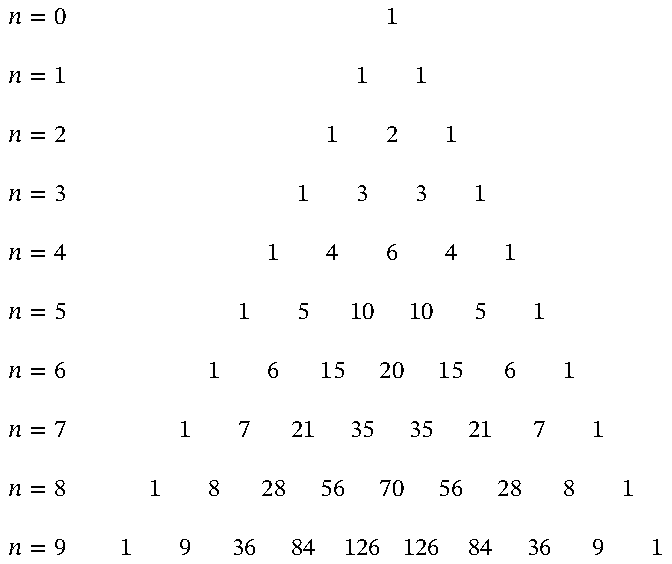
\includegraphics[scale=1]{./tex-images/thap-he-so-nhi-thuc-den-n-bang-9/thap-he-so-nhi-thuc-den-n-bang-9.pdf}
    \caption{Trong các văn bản toán học, tháp này thường được gọi là tam giác Pascal, xem \cite{edwards2019pascal}.}
    \label{fig:thap-he-so-nhi-thuc-den-n-bang-9}
\end{figure}

\begin{figure}[htbp]
    \centering
    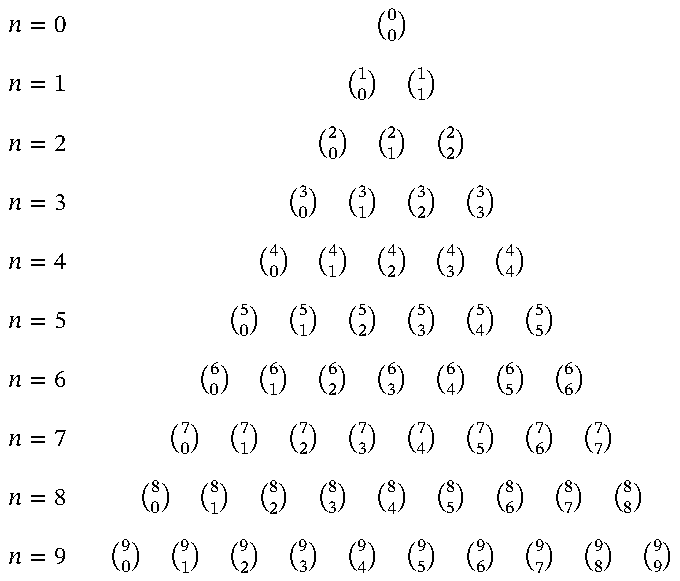
\includegraphics[scale=1]{./tex-images/thap-he-so-nhi-thuc-dang-ki-hieu-den-n-bang-9/thap-he-so-nhi-thuc-dang-ki-hieu-den-n-bang-9.pdf}
    \caption{Tháp mười dòng hệ số đầu tiên dạng kí hiệu.}
    \label{fig:thap-he-so-nhi-thuc-dang-ki-hieu-den-n-bang-9}
    % \label{fig:example}
\end{figure}
Tháp trong \autoref{fig:thap-he-so-nhi-thuc-den-n-bang-9} còn có thể mở rộng vô hạn về phía đáy chỉ bằng cách sử dụng phép cộng để viết tiếp các \(p_{10}\), \(p_{11}\), vân vân. Tuy nhiên, khi \(n\) tăng lên, khối lượng cần ghi chú ngày càng lớn, điều này bộc lộ hạn chế khi muốn viết một \(p_n\) với \(n\) lớn. Như đã thấy, tôi cần viết từ \(p_0\) đến \(p_8\) trước khi có thể viết \(p_9\), và tương tự, cần viết từ \(p_0\) đến \(p_{n-1}\) trước khi viết \(p_n\). Về mặt lí thuyết, điều này có thể thực hiện được, nhưng trong thực tế, công việc trở nên quá phức tạp khi \(n\) lớn, mặc dù chỉ đơn giản là phép cộng và ghi chú. 

Để công việc nhẹ nhàng hơn, tôi tự hỏi liệu có cách nào để viết trực tiếp \(p_n\) hay không? Cụ thể hơn, liệu có tồn tại công thức tính \(\binom{n}{j}\) thông qua \(\binom{n}{j-1}\) hay không?

Quan sát dãy hệ số của \(p_5\) gồm \(\binom{5}{0}=1, \binom{5}{1}=5, \binom{5}{2}=10, \binom{5}{3}=10, \binom{5}{4}=5, \binom{5}{5}=1\). Lấy các hệ số này nhân với các số mũ tương ứng của \(x\), sẽ thu được kết quả như ở cột bên trái dưới đây. Mặt khác, theo công thức \eqref{eq:tinh-doi-xung}, từ cột bên trái, tôi cũng viết được cột bên phải. 
\begin{align*}
    \begin{aligned}
        0\cdot\binom{5}{0}&=0 \\
        1\cdot\binom{5}{1}&=5 \\
        2\cdot\binom{5}{2}&=20 \\
        3\cdot\binom{5}{3}&=30 \\
        4\cdot\binom{5}{4}&=20 \\
        5\cdot\binom{5}{5}&=5
    \end{aligned}
    \hspace{2cm}
    \begin{aligned}
        (5-5)\cdot\binom{5}{5}&=0 \\
        (5-4)\cdot\binom{5}{4}&=5 \\
        (5-3)\cdot\binom{5}{3}&=20 \\
        (5-2)\cdot\binom{5}{2}&=30 \\
        (5-1)\cdot\binom{5}{1}&=20 \\
        (5-0)\cdot\binom{5}{0}&=5
    \end{aligned}
\end{align*}
Bây giờ, tôi bỏ đi dòng đầu tiên của cả hai cột và viết nghịch đảo lại cột bên phải, tôi thu được hai cột như dưới đây.
\begin{align*}
    \begin{aligned}
        1\cdot\binom{5}{1}&=5 \\
        2\cdot\binom{5}{2}&=20 \\
        3\cdot\binom{5}{3}&=30 \\
        4\cdot\binom{5}{4}&=20 \\
        5\cdot\binom{5}{5}&=5
    \end{aligned}
    \hspace{2cm}
    \begin{aligned}
        (5-0)\cdot\binom{5}{0}&=5 \\
        (5-1)\cdot\binom{5}{1}&=20 \\
        (5-2)\cdot\binom{5}{2}&=30 \\
        (5-3)\cdot\binom{5}{3}&=20 \\
        (5-4)\cdot\binom{5}{4}&=5 
    \end{aligned}
\end{align*}

Từ quan sát như vậy, tôi đưa ra giả thiết qui nạp là, với \(1\leq j \leq n\), 
\begin{align}
    j\binom{n}{j}=(n-j+1)\binom{n}{j-1}. \label{eq:tinh-he-so-nhi-thuc-theo-chieu-ngang}
\end{align}
Cơ sở qui nạp là bất kì trường hợp nào được liệt kê trong tháp hệ số ở \autoref{fig:thap-he-so-nhi-thuc-den-n-bang-9}, cũng như trường hợp vừa xét qua ở trên, các hệ số của \(p_5\).

Sử dụng công thức \eqref{eq:tinh-he-so-nhi-thuc-theo-chieu-doc} kết hợp với giả thiết qui nạp là công thức \eqref{eq:tinh-he-so-nhi-thuc-theo-chieu-ngang} để có hai phép biến đổi
\begin{align*}
    \binom{n+1}{j} 
        &= \binom{n}{j-1}+\binom{n}{j} \\
        &= \binom{n}{j-1}+\frac{n-j+1}{j}\binom{n}{j-1} \\
        &= \frac{n+1}{j}\binom{n}{j-1}
\end{align*}
và\begin{align*}
    \binom{n+1}{j-1}\frac{n-j+2}{j} 
        &= \left[\binom{n}{j-2}+\binom{n}{j-1} \right] \frac{n-j+2}{j} \\
        &= \left[\frac{j-1}{n-j+2}\binom{n}{j-1}+\binom{n}{j-1} \right] \frac{n-j+2}{j} \\
        &= \frac{n+1}{j}\binom{n}{j-1}.
\end{align*}
Từ đây, suy ra kết luận qui nạp là
\[ j\binom{n+1}{j} = (n-j+2)\binom{n+1}{j-1}.\,\square\]

Để xây dựng tháp hệ số như trong \autoref{fig:thap-he-so-nhi-thuc-den-n-bang-9}, công thức \eqref{eq:tinh-he-so-nhi-thuc-theo-chieu-doc} cho phép tôi tiến hành theo chiều dọc và công thức \eqref{eq:tinh-he-so-nhi-thuc-theo-chieu-ngang} cho phép tôi tiến hành theo chiều ngang. Nương theo chiều hướng suy luận như thế, một câu hỏi hợp lí phát sinh là liệu có thể tiến hành theo các đường chéo được hay không? Diễn đạt toán học cho câu hỏi này là liệu có thể tính được \(\binom{n}{j}\) hoặc thông qua \(\binom{n-1}{j-1}\) - đường chéo hướng từ trái sang phải, hoặc thông qua \(\binom{n-1}{j}\) - đường chéo còn lại, hay không? Câu trả lời là có thể, bạn hãy xem
\begin{align*}
    \binom{n}{j} 
        &= \binom{n-1}{j-1}+\binom{n-1}{j} \\
        &= \binom{n-1}{j-1}+\frac{n-j}{j}\binom{n-1}{j-1} \\
        &= \frac{n}{j}\binom{n-1}{j-1}
\end{align*}
và
\begin{align*}
    \binom{n}{j} 
        &= \binom{n-1}{j-1}+\binom{n-1}{j} \\
        &= \frac{j}{n-j}\binom{n-1}{j}+\binom{n-1}{j} \\
        &= \frac{n}{n-j}\binom{n-1}{j}.\,\square
\end{align*}

Vậy, tôi kết luận
\begin{align}
    \binom{n}{j}=\frac{n}{j}\binom{n-1}{j-1} \label{eq:tinh-he-so-nhi-thuc-theo-duong-cheo-trai}
\end{align}
và
\begin{align}
    \binom{n}{j}=\frac{n}{n-j}\binom{n-1}{j}. \label{eq:tinh-he-so-nhi-thuc-theo-duong-cheo-phai}
\end{align}

Quan sát các bước biến đổi dẫn đến hai đẳng thức trên, tôi thấy rằng phép dựng, tháp hệ số nhị thức, theo đường chéo là sự kết hợp của hai phép dựng theo chiều dọc và chiều ngang. Ý tưởng này có thể được áp dụng và mở rộng vào những cấu trúc toán học khác, giúp giải quyết các vấn đề một cách sáng tạo và hiệu quả. Chẳng hạn, với các số Sì-tớ-liềng\footnote{Stirling} loại hai, tôi có thể thấy những tính chất tương tự như với các hệ số nhị thức hay không? Việc nghiên cứu theo hướng này đôi khi mang lại những kết quả thú vị trong toán học.

Quay trở lại với vấn đề đang cần giải quyết, tôi đặt ra câu hỏi sâu hơn liệu có một công thức tổng quát để tính \(\binom{n}{j}\) chỉ phụ thuộc vào \(n\) và \(j\) mà không cần dựa vào các hệ số khác hay không? 

Câu hỏi này quan trọng bởi nếu có một công thức tổng quát như vậy, tôi có thể tính trực tiếp hệ số nhị thức mà không cần sử dụng các hệ số nhị thức khác làm trung gian. Điều này sẽ giúp tiết kiệm thời gian và công sức, đặc biệt là khi làm việc với các hệ số nhị thức lớn. Hơn nữa, một công thức tổng quát như vậy sẽ cung cấp một cái nhìn sâu sắc hơn về bản chất của các hệ số nhị thức và mối quan hệ giữa chúng với \(n\) và \(j\).

Căn cứ vào công \eqref{eq:tinh-he-so-nhi-thuc-theo-duong-cheo-trai}, xét phép biến đổi 
    \begin{align*}
        \binom{n}{j} 
                &= \frac{n}{j}\binom{n-1}{j-1} \\
                &= \frac{n}{j}\frac{n-1}{j-1}\binom{n-2}{j-2} \\
                &= \frac{n}{j}\frac{n-1}{j-1} \cdots \frac{n-j+1}{1}\binom{n-j}{0} \\
                &= \frac{n(n-1)\cdots (n-j+1)}{j(j-1)\cdots 1}.
    \end{align*}
Với các công thức \eqref{eq:tinh-he-so-nhi-thuc-theo-chieu-doc}, \eqref{eq:tinh-he-so-nhi-thuc-theo-chieu-ngang}, \eqref{eq:tinh-he-so-nhi-thuc-theo-duong-cheo-trai} và \eqref{eq:tinh-he-so-nhi-thuc-theo-duong-cheo-phai}, tôi có thể tính một hệ số nhị thức thông qua các hệ số nhị thức khác ở xung quanh. Nhưng với công thức vừa tìm được, tôi có thể tính trực tiếp một hệ số nhị thức chỉ cần biết vị trí của nó trong tháp ở \autoref{fig:thap-he-so-nhi-thuc-dang-ki-hieu-den-n-bang-9}. Nói cách khác là bây giờ tôi đã có thể tính được hệ số của bất kì \(x^j\) với \(0\leq j \leq n\) khi khai triển \((1+x)^n\) với \(n\) tùy ý. Ví dụ, hệ số của \(x^6\) khi khai triển \((1+x)^9\) là
\[\binom{9}{6}=\frac{9\cdot 8\cdot 7\cdot 6\cdot 5 \cdot 4}{6\cdot 5\cdot 4\cdot 3\cdot 2\cdot 1}=84.\]
Hãy đối chiều kết quả này với hạng tử thứ bảy thuộc dòng thứ mười trong tháp ở \autoref{fig:thap-he-so-nhi-thuc-den-n-bang-9} để xác nhận kết quả.

Định nghĩa \(n!=n\cdot (n-1)\cdots 1\), gọi \(n!\) là \(n\) \emph{giai thừa}, để viết công thức tính hệ số nhị thức vừa tìm được thành dạng
\begin{align}
    \binom{n}{j} = \frac{n!}{j!(n-j)!}. \label{eq:tinh-he-so-nhi-thuc}
\end{align}

Câu trả lời trên không chỉ chính xác mà còn bất ngờ vì nó cho thấy rằng các hệ số nhị thức thực sự liên quan đến một công thức có ý nghĩa quan trọng trong lí thuyết tổ hợp. Cụ thể, \(\binom{n}{j}\) còn được biết đến khi cần đếm số tập con \(j\) phần tử của tập \(n\) phần tử, hay số cách chọn \(j\) phần tử không kể thứ tự từ \(n\) phần tử. Do đó tôi có thể gọi \(\binom{n}{j}\) là ``\(n\) chọn \(j\)'' hay số \emph{tổ hợp} chập \(j\) của \(n\). Vì sao lại có mối liên hệ này giữa hệ số nhị thức và số tổ hợp?

Ví dụ, trong khai triển \((1+x)^3=\binom{3}{0}+\binom{3}{1}x+\binom{3}{2}x^2+\binom{3}{3}x^3\), hệ số \(\binom{3}{2}\) chính là số lượng \(x^2\) có trong tích \((1+x)(1+x)(1+x)\). Mặt khác, nó cũng có thể được hiểu là số cách chọn hai phần tử \(x\) từ ba phần tử là các thừa số ở vế trái để viết một hạng tử là tích ba thừa số ở vế phải, bao gồm hai thừa số \(x\) và một thừa số \(1\). Điều này thể hiện qua cách viết khai triển chưa rút gọn của \((1+x)^3\) như sau
\begin{align*}
    (1+x) \cdot (1+x) \cdot (1+x)
        & = 1 \cdot 1 \cdot 1 + x \cdot 1 \cdot 1 + 1 \cdot x \cdot 1 \\
        & \qquad + x \cdot x \cdot 1 + 1 \cdot 1 \cdot x + x \cdot 1 \cdot x + 1 \cdot x \cdot x + x \cdot x \cdot x.
\end{align*}
Tổng quát, \(\binom{n}{j}\) là số cách chọn \(j\) phần tử \(x\) từ \(n\) phần tử là các thừa số của tích 
\[\underbrace{(1+x)(1+x)\cdots(1+x)}_{\text{có \(n\) thừa số}}.\]

\begin{baitap}
Một tập hợp có \(n\) phần tử thì có bao nhiêu tập con, kể cả tập rỗng và chính nó?
\end{baitap}

%%%%%%%%%%

\section{Định lí nhị thức}

Giờ đây tôi đã có đủ chất liệu để phát biểu định lí nhị thức, tổng hợp lại những kiến thức đã phát hiện được trong quá trình khai triển lũy thừa \((1+x)^n\) đã tiến hành ở trên. 

Lũy thừa nguyên không âm \(n\) của nhị thức \(1+x\) được khai triển thành tổng có dạng 
\[(1+x)^n=\binom{n}{0}+\binom{n}{1}x+\cdots+\binom{n}{n-1}x^{n-1}+\binom{n}{n}x^n\]
hoặc viết dưới dạng tổng xích-mờ là
\[(1+x)^n=\sum_{j=0}^n\binom{n}{j}x^n.\]
Trong đó, \(\binom{n}{j}\) được gọi là các hệ số nhị thức và được xác định bằng công thức 
\[\binom{n}{j}=\frac{n!}{j!(n-j)!}=\frac{n(n-1)\cdots(n-j+1)}{j(j-1)\cdots 1},\]
với qui ước \(0!=1\). Các hệ số nhị thức này có các tính chất
\begin{align*}
    \binom{n}{j}&=\binom{n-1}{j-1}+\binom{n-1}{j}, \\
    \binom{n}{j}&=\binom{n}{n-j}, \\
    \binom{n}{j}&=\frac{n-j+1}{j}\binom{n}{j-1},\\
    \binom{n}{j}&=\frac{n}{j}\binom{n-1}{j-1}, \\
    \binom{n}{j}&=\frac{n}{n-j}\binom{n-1}{j}.
\end{align*}

\begin{baitapcham}
    Bạn hãy chứng minh lại các đẳng thức trên bằng công thức tính hệ số nhị thức mới tìm được.
\end{baitapcham}

Như đã đề cập ở \autoref{sec:dan-nhap}, nếu \(x\ne 0\), tôi có thể khai triển lũy thừa \((x+y)^n\) bằng cách áp dụng dạng khai triển của \((1+x)^n\) như sau
\begin{align*}
    (x+y)^n 
        &= x^n\left[1+\left(\frac{y}{x}\right)\right]^n \\
        &= x^n\sum_{j=0}^n \binom{n}{j}\left(\frac{y}{x}\right)^j \\
        &=\sum_{j=0}^n\binom{n}{j}x^{n-j}y^j.
\end{align*}
Mặt khác, do \(x\) và \(y\) có vai trò như nhau trong biểu thức \((x+y)^n\) nên có thể viết
\[(x+y)^n=\sum_{j=1}^n\binom{n}{j}x^jy^{n-j}.\]
Đây là phiên bản quen thuộc và thường được sử dụng khi trình bày định lí nhị thức.

\begin{baitap}
    \begin{enumerate}
        \item Chứng minh \(\binom{2n}{0}-\binom{2n}{2}+\binom{2n}{4}-\cdots +(-1)^{2n-2}\binom{2n}{2n-2}+(-1)^{2n}\binom{2n}{2n}=2^n\cos{\frac{n\pi}{2}}\). Sự hiện diện của \(\cos{\frac{n\pi}{2}}\) trong đẳng thức này gợi lên trong bạn những suy nghĩ gì? 
        \item Cho \(n\) là số nguyên không âm, chứng minh rằng khi \(n\) tăng vô hạn, \(\sum_{j=0}^n\frac{1}{j!}\) và \(\left(1+\frac{1}{n}\right)^n\) cùng hội tụ về một giới hạn. Được biết giới hạn đó chính là số \(\operatorname{e}=2,718\ldots\).
    \end{enumerate}
\end{baitap}

%%%%%%%%%

% THƯ MỤC
\printbibliography

\end{document}
